\section{Реализация моделей}
	В данном разделе приводится краткое описание программной реализации
	моделей, примеры рассчитанных частотных сканов, примеры результатов
	идентификации их моделей.


	\subsection{Интерфейс и функционал}
	Модели оформлены в виде пакета модулей на языке программирования Python~3.
	Интерфейс моделей совместим с одной из самых популярных библиотек для 
	машинного обучения scikit-learn \cite{sklearn_website}. Такое техническое
	решение позволяет использовать имеющиеся в библиотеке инструменты 
	предобработки данных, оценки качества моделей и оптимизации параметров 
	моделей, а также интегрировать модели в друге программное обеспечение и 
	конвейеры обработки данных.

	Разработанные модели (выражения	\ref{eq:dls82e_model_S_short}, 
	\ref{eq:dls82e_model_S_p}, \ref{eq:multiexp_frequncy_scan}), выполняют две 
	функции:
	\begin{enumerate}
		\item Вычисление частотного скана с заданными параметрами.
		\item Идентификация параметров модели частотного скана по 
		экспериментальным данным.
	\end{enumerate}
	Идентификация параметров моделей реализована методом градиентного спуска.
	Имеется возможность вывода значений параметров модели на каждой итерации.
	Реализована автоматическая остановка идентификации при достижении заданного
	модуля разницы между значениями функции потерь на текущей и предыдущей 
	итерации.

	Модели реализуют единообразный интерфейс. При инициализации каждая модель 
	получает длительность импульса заполнения (параметр filling\_pulse),
	которая считается неизменной при измерениях) и параметры алгоритма 
	идентификации. Параметры алгоритма идентификации варьируются:
	\begin{itemize}
		\item модель идеального частотного скана и модель частотного скана с 
		показателем нелинейности-неэкспоненциальности (выражения 
		\ref{eq:dls82e_model_S_short}, \ref{eq:dls82e_model_S_p}): 
			\begin{description}
				\item[fit\_p\_coef] -- если параметр принимает значение True 
				(логическую единицу), тогда при идентификации параметров модели
				определяется показатель нелинейности-неэкспоненциальности $p$,
				иначе (False -- логический ноль) $p$ считается равным 1 при 
				идентификации параметров модели;
				\item[learning\_rate] -- скорость градиентного спуска;
				\item[n\_iters] -- максимальное количесво итераций при 
				идентификации;
				\item[stop\_val] -- модуль разницы между значениями функции 
				потерь на текущей и предыдущей итерации, при достижении которого
				происходит остановка идентификации;
				\item[verbose] -- если параметр принимает значение True, то в 
				статдартный поток вывода печатаются значения параметров модели
				на каждой итерации.
			\end{description}

		\item модель многоэкспоненциального частотного скана (выражение 
		\ref{eq:multiexp_frequncy_scan}):
			\begin{description}
				\item[n\_exps] -- количество экспоненециальных составляющих в 
				сигнале релаксации (значение $n$ в выражении 
				\ref{eq:multiexp_frequncy_scan});
				\item[learning\_rate] -- скорость градиентного спуска;
				\item[n\_iters] -- максимальное количесво итераций при 
				идентификации;
				\item[stop\_val] -- модуль разницы между значениями функции 
				потерь на текущей и предыдущей итерации, при достижении которого
				происходит остановка идентификации;
				\item[verbose] -- если параметр принимает значение True, то в 
				статдартный поток вывода печатаются значения параметров модели
				на каждой итерации.
			\end{description}
	\end{itemize}

	При идентификации параметров модели идеального частотного скана 
	определяется амплитуда и десятичный логарифм постоянной времени 
	($\log_{10}(\tau)$) сигнала релаксации. Причины замены постоянной времени
	её десятичном логарифмом объясняются в следующем разделе.

	При идентификации модели с показателем нелинейности"=неэкспоненциальности
	к амплитуде и десятичному логарифму постоянной времени сигнала релаксации
	добавляется значение показателя нелинейности"=неэкспоненциальности $p$.

	При идентификации многоэкспоненциальной модели определяется $n$ пар 
	амплитуда --- десятичный логарифм постоянной времени сигнала релаксации. 
	По паре для каждой из $n$ экспоненциальных составляющих.

	Параметры модели частотного скана могут быть не только идентифицированны,
	но и заданы пользователем.

	Чтобы выполнить идентификацию параметров модели, нужно передать ей 
	набор экспериментальных (тренировачных) данных, состоящих из вектора 
	значений десятичных логарифимов частоты опорной функции ($\log_{10}(F_0)$)
	и соответствующего вектора значений сигнала DLTS -- сигнала на выходе 
	аппаратного тракта спектрометра DLS-82E. При идентификации параметров модели
	по умолчанию их начальные параметры выбираются случайным образом, однако
	могут быть и определены пользователем.

	При идентификации модели значения её параметров на каждой итерации 
	сохраняются в атрибуте fit\_results\_, что позволяет пользователю
	получить и проанализировать данные о работе алгоритма идентификации.

	При вычислении частотного скана с заданными параметрами модели передаётся
	вектор значений десятичных логарифимов частоты опорной функции, для каждого 
	из которых модель вычислит значение сигнала	DLTS.


	\subsection{Алгоритм идентификации параметров моделей}
	Идентификация параметров модели производится методом градиетного 
	спуска, при этом минимизируется среднеквадратическая ошибка между 
	значениями, полученными в результате измерений, и результатами 
	моделирования (выражение \ref{eq:mse}).
	\begin{equation}
		\label{eq:mse}
		E = \frac{1}{m}\sum_{i=1}^{m}\left(y_i - y_i^*\right)^2,
	\end{equation}
	где
	\begin{description}
		\item[$y_i$] -- значения, полученные в результате измерений,
		\item[$y_i^*$] -- значения, полученные в результате моделирования,
		\item[$m$] -- количество измерений.
	\end{description}
	При этом при каждом обновлении постоянной времени сигнала релаксации 
	(как при идентификации модели, на каждой итерации, так и при обновлении
	постоянной времени пользователем) вычисляется масштабный множитель 
	$M(\tau, F_0, t_1)$, определяемый выражением \ref{eq:dls82e_model_M}.
	Таким образом модель всякий раз вычисляет значение 	
	\(
		\max{\left[
	    \tau F_0 e^{-\frac{0.05}{\tau F_0}}
	    \left(1-e^{\frac{t_1 F_0-0.45}{\tau F_0}}
	    -e^{-\frac{0.5}{\tau F_0}}+
	    e^{\frac{t_1 F_0-0.95}{\tau F_0}}\right)
	    \right]}
    \).
    
    В текущей реализации моделей данный максимум вычисляется приблизительно
    с помощью градиентного спуска. Не смотря на то, что применяемый итеративный
    алгоритм находит максимум очень быстро, эти вычисления занимают довольно 
    много веремени при идентификации моделей, потому что выполняются на 
    каждой итерации (при каждом обновлений постоянной времени $\tau$). А в 
    случае многоэкспоненциальной модели данный процесс повторяется еще и для 
    каждой экспоненциальной составляющей, что заметно снижает скорость
    идентификации модели при n\_exps > 10. Таким образом в будущем вычисления 
    можно будет оптимизировать за счёт одного из следющих решений:
    \begin{enumerate}
    	\item найти точное аналитическое выражение для расчёта $M$,
    	\item найти для $M(\tau, F_0, t_1)$ аппроксимирующую функцию, 
    	позволяющую вычислять мастабный множитель с приемлимой точностью.
    \end{enumerate}

	В моделях градиентный спуск реализован при помощи библиотеки TensorFlow
	\cite{tf_website}, главное преимущество которой в том, что она реализует
	алгоритм автоматического дифференцирования на графе вычислений. Таким 
	образом, при расчёте градиентов сначала производные берутся символьно 
	(точно), а затем вычисляются их значения, поэтому точность вычисления 
	градиента ограничена только разрядностью чисел \cite{hands_on_ml},
	\cite{nikolenko_deep_learning}, \cite{tf_website}.



	

    \begin{figure}[!ht]
        \centering
        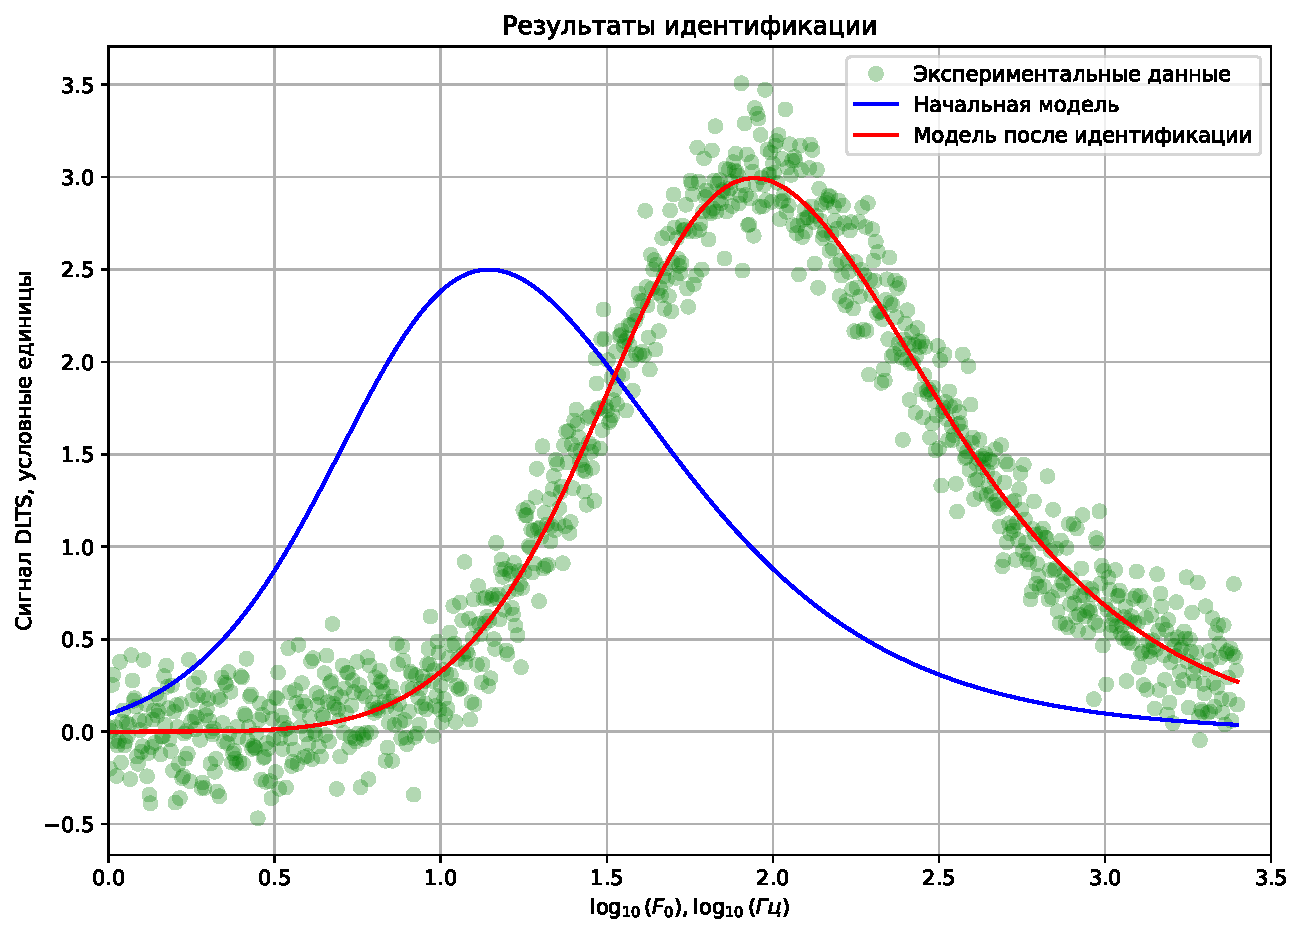
\includegraphics[width=0.75\textwidth]{identification_test}
        \caption{Пример результата идентификации модели идеального частотного 
        скана.}
        \label{pic:identification_test}
    \end{figure}


    \begin{figure}[!ht]
        \centering
        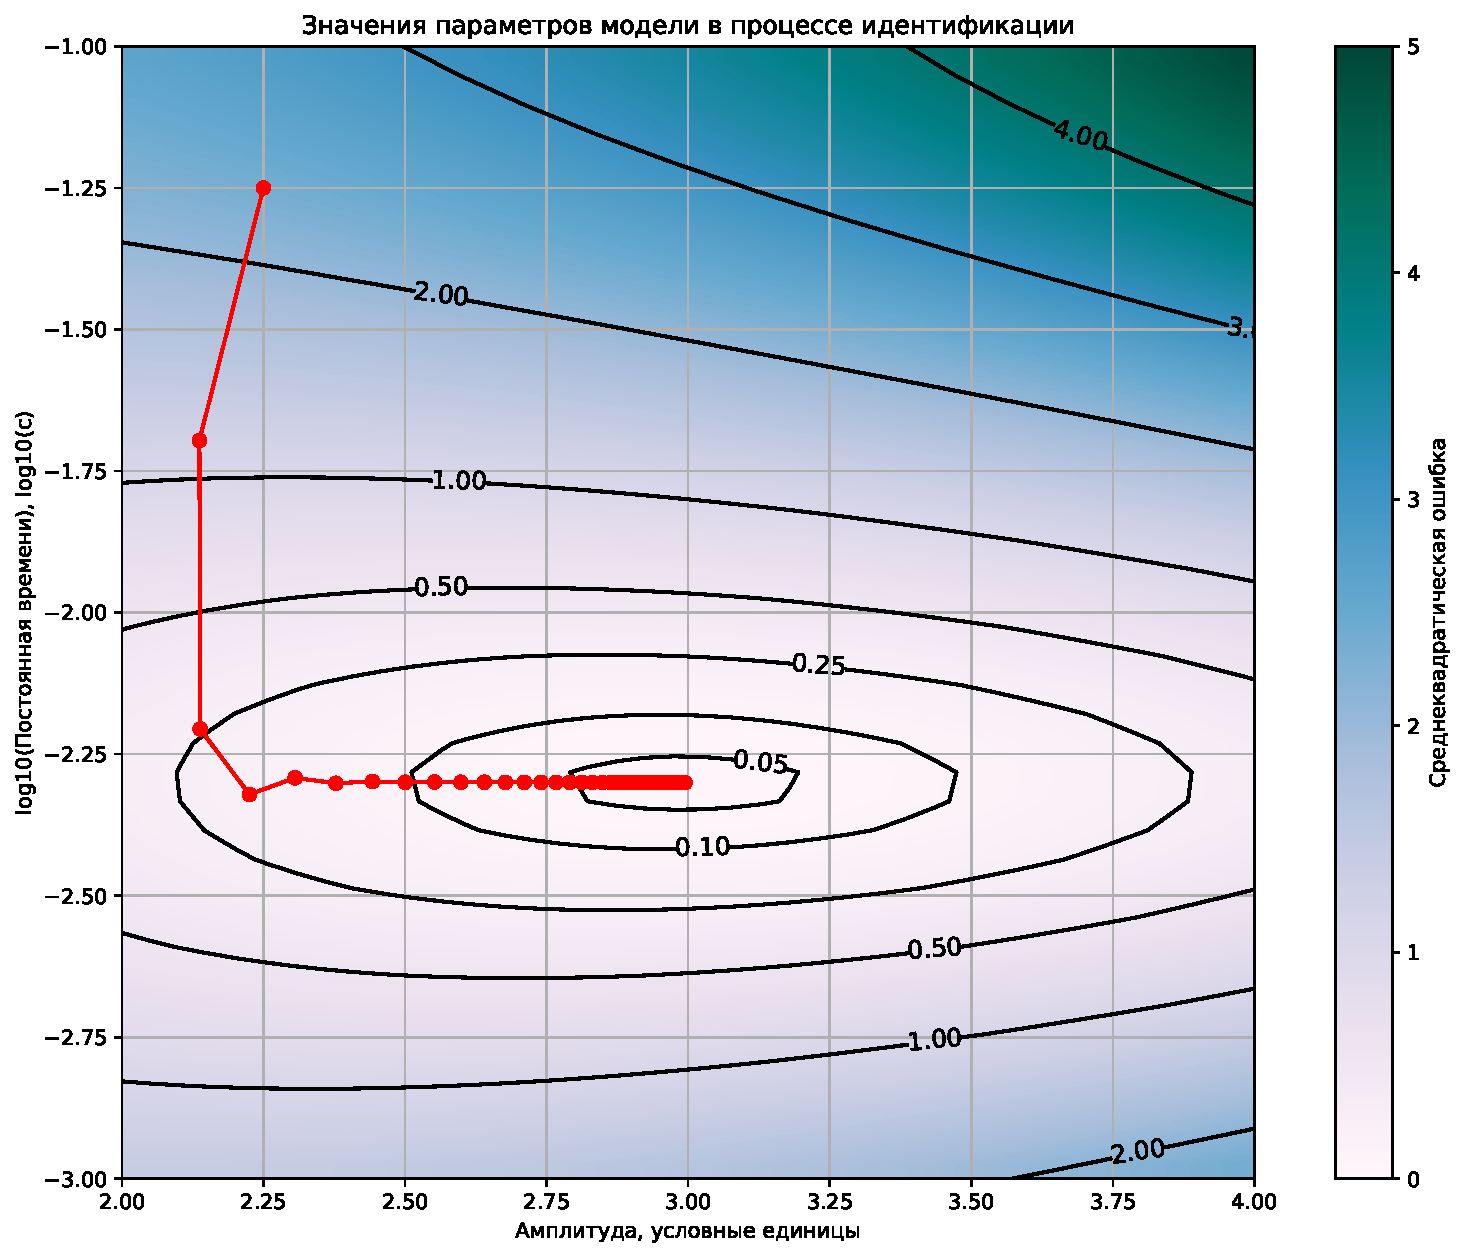
\includegraphics[width=0.75\textwidth]{path}
        \caption{<<Путь>> значений параметров при идентификации.}
        \label{pic:path}
    \end{figure}


    \begin{figure}[!ht]
        \centering
        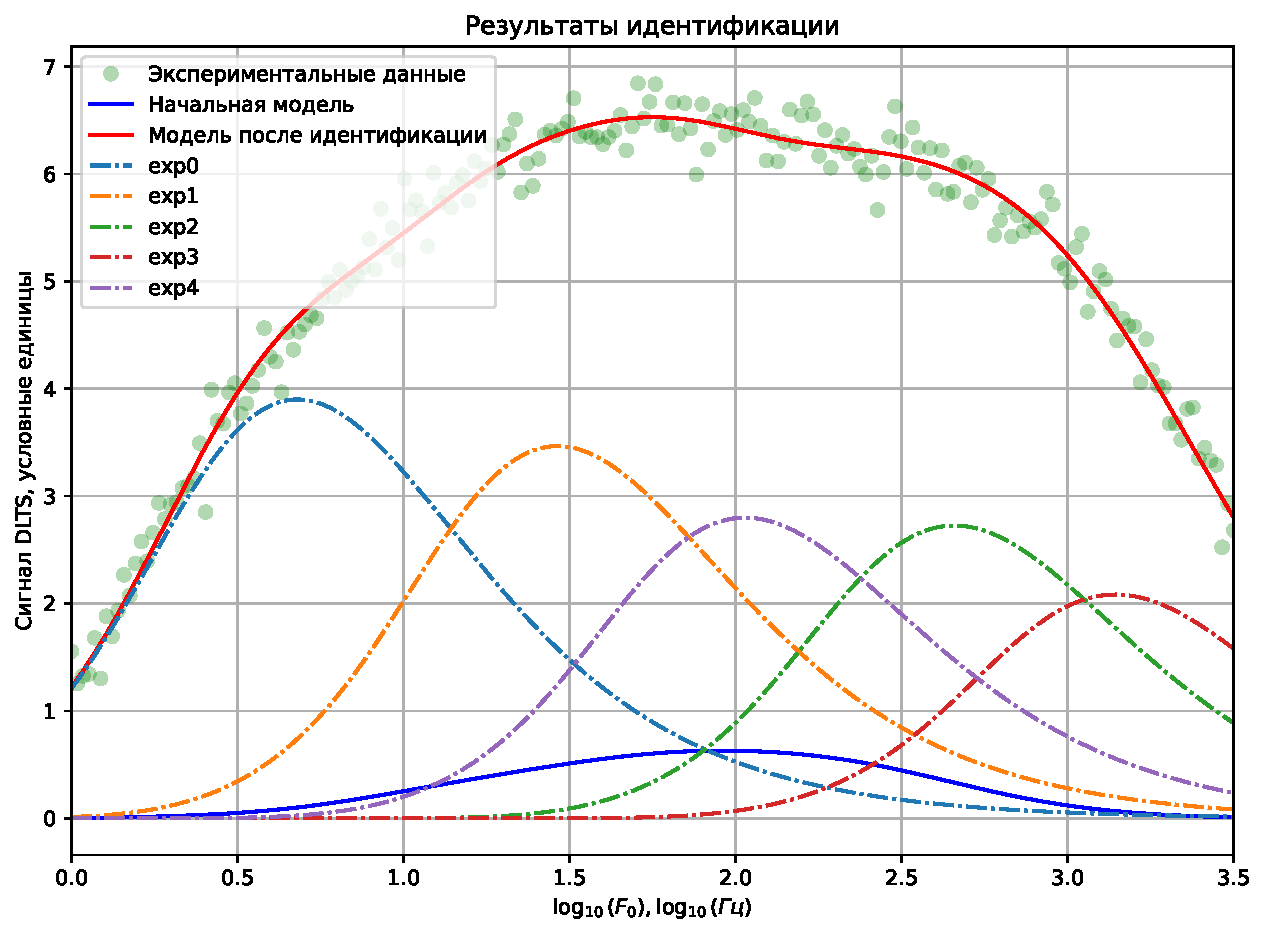
\includegraphics[width=0.75\textwidth]{multiexp_test}
        \caption{Пример результата идентификации модели многоэкспоненциального
        частотного скана.}
        \label{pic:multiexp_test}
    \end{figure}


    \subsection{Оценка качества модели}
    Несколько слов о рабочем процессе при разработке моделей, идентификации
    их параметров, оптимизации параметров алгоритма идентификации.

    Про идентификацию, градиентный спуск, нормализацию ...

    Иллюстрации оверфитинга.